% !TEX root = slides_ISSTA.tex

\subsection{Examples}

\begin{frame}[fragile]
\frametitle{Regular Expressions: The Basics}

\begin{Large}
\begin{columns}

\begin{column}{0.4\textwidth}
\begin{itemize}
\item \cverb!(ab*c|yz*)$!
	\begin{itemize}
		\item[\Checkmark] abbbbbbbc
		\vspace{6pt}	
		\item[\Checkmark] y
		\vspace{6pt}	
		\item[\Checkmark] abcy	
		\vspace{12pt}	
		\item[\XSolidBrush] \onslide<2->{abcccc }
		\vspace{6pt}			
		\item[\XSolidBrush] \onslide<2->{yxw}
	\end{itemize}
\end{itemize}
\end{column}

\begin{column}{0.4\textwidth}
\onslide<3->
\begin{itemize}
	\item\cverb!(ab*c|yz*)!
\onslide<4->
	\begin{itemize}
		\item[\Checkmark] abbbbbbbc
		\vspace{6pt}		
		\item[\Checkmark] y
		\vspace{6pt}
		\item[\Checkmark] abcy	
		\vspace{12pt}	
		\item[\Checkmark] {abcccc }
		\vspace{6pt}		
		\item[\Checkmark] {yxw}
	\end{itemize}
	
	\end{itemize}
	
\end{column}
\end{columns}
\end{Large}
\end{frame}
%------------------------------------------------

\begin{frame}
\frametitle{In Python: Utilizations of the re module}
\begin{figure}[h]
  \centering
  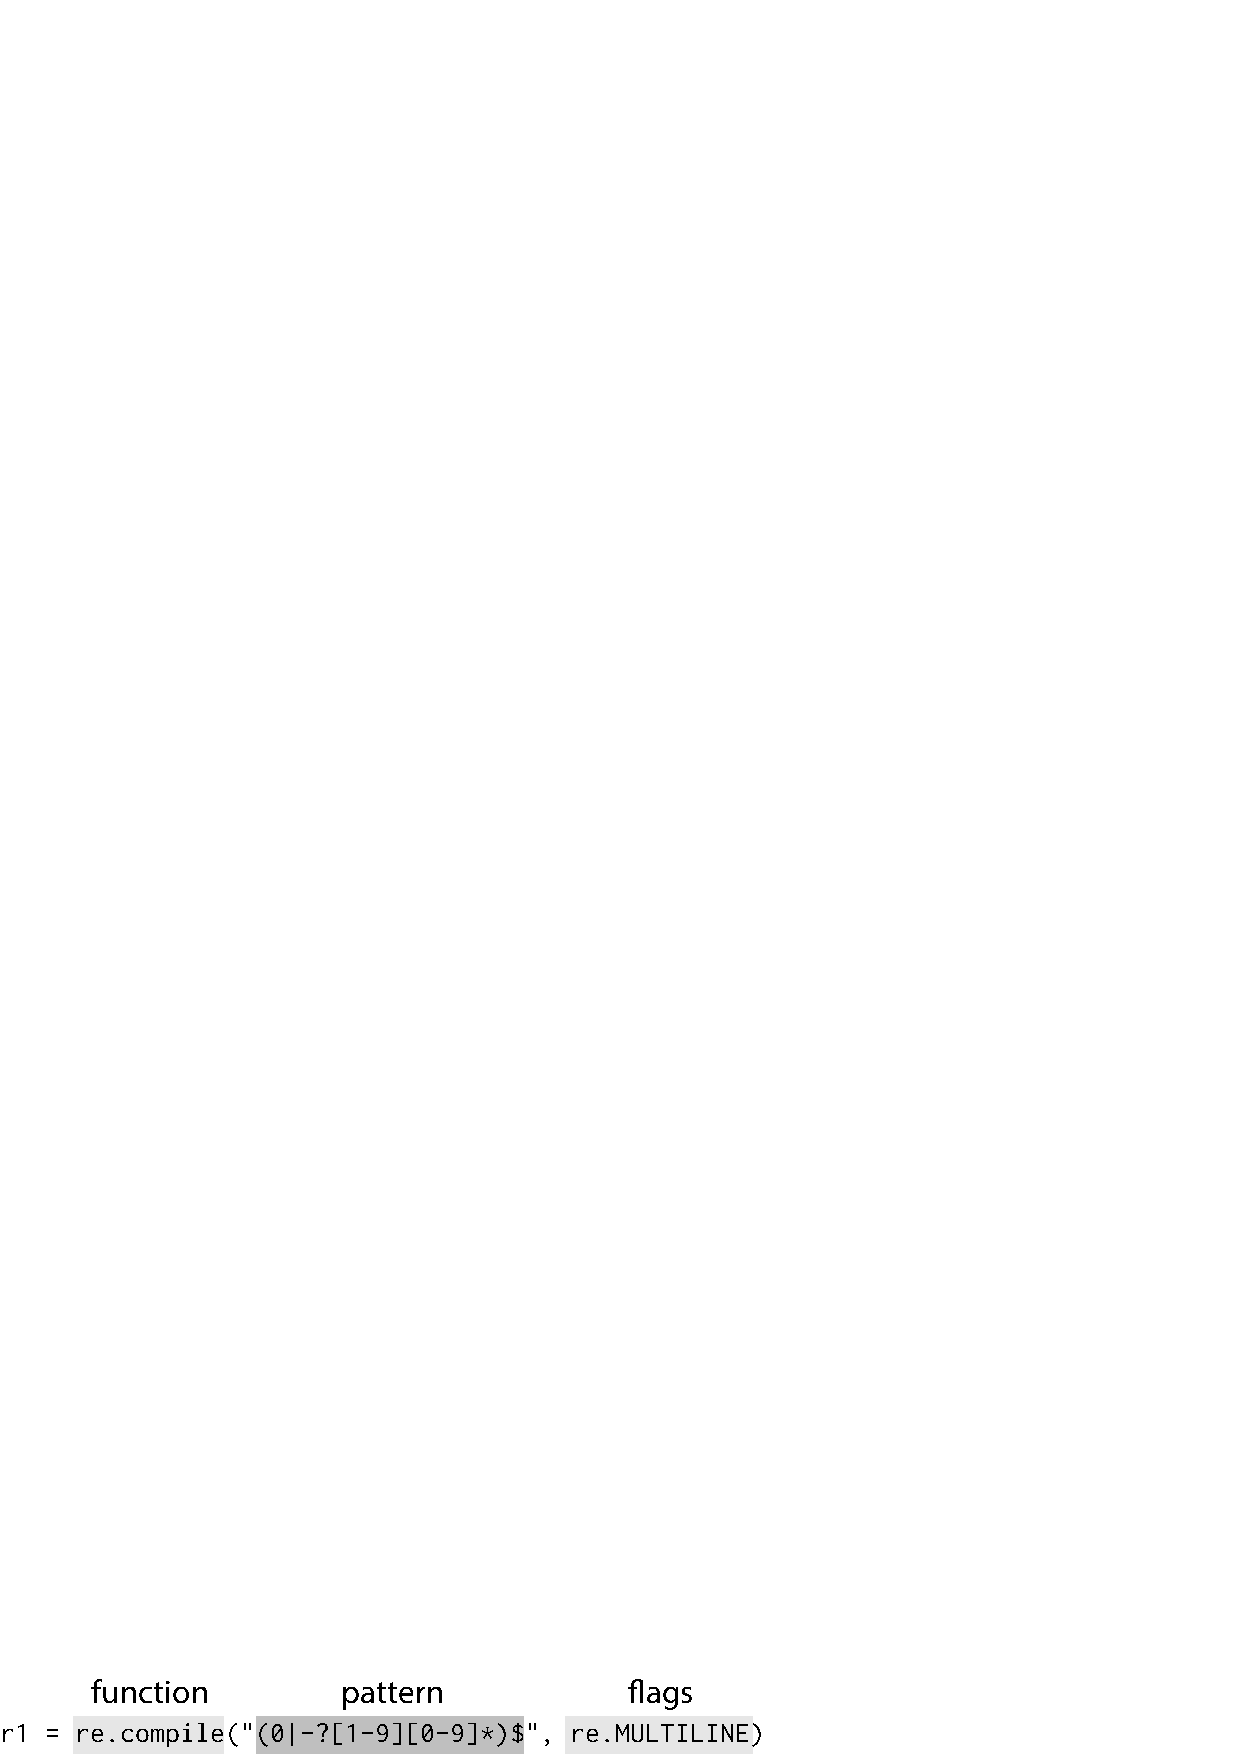
\includegraphics[scale=0.77]{../nontex/illustrations/exampleUsageLarge.pdf}
  \label{fig:exampleUsageLarge}
\end{figure}
\begin{description}
\item [function] which function of the re module is called?
\item [pattern] string used to specify regex behavior
\item [flags] modifies the regex engine
\end{description}
\end{frame}
\note[itemize]{
    \item 53,894 unique utilizations observed.
    \item pt 2
}

